\section { Computer Vision }
	\subsection { Kameraparameter }
	\subsection { Segmentierung }
		

	
\section { Machine Learning }
	In den letzen Jahren gab es stetige Fortschritte in der Leistungsfähigkeit von Rechenhardware und damit einhergehend im Bereich des maschinellen Lernens (en. machine learning).
	In diesem Abschnitt werden kurz die in der Arbeit genutzten machine-learning Techniken aufgezeigt und erläutert.
	
	\subsection { Neuronale Netze }
	Künstliche Neuronale Netze (en.: artificial neural networks, kurz: ANN) sind der biologischen Funktionsweise menschlicher Nervenbahnen nachempfunden. 
	
		\subsubsection { Das Perzeptron }
		Das einlagige Perzeptron, der einfachste Fall eines neuronalen Netzes, besteht aus drei Schichten von jeweils beliebig vielen Recheneinheiten, die als Neuronen bezeichnet werden. Alle Neuronen sind dabei mit allen Neuronen der nachfolgenden Schicht über eine gewichtete Verbindung verknüpft. 
		
		Die erste Schicht übernimmt im einlagigen Perzeptron die Rolle des Eingangs. Die zweite Lage wird als "`hidden layer"' bezeichnet und die dritte Schicht stellt die berechneten Ausgangsdaten zur Verfügung.
		
		Jede Recheneinheit nimmt die Daten $o_{j-1} = o_i$ aus den vorhergehenden Neuronen entgegen und berechnet einen vorläufigen Ausgangswert $p_j$ nach Gleichung \ref{eq:perceptron_simple}. 
		
		\begin{equation}
			\label{eq:perceptron_simple}
			\text{net}_j = \sum_{i=1}^{n} w_{ij} \cdot o_i + b
		\end{equation}
		
		Die Gewichte $w_{xy}$ und Bias-Werte $b_x$ werden im Trainingsprozess anhand der Trainingsdaten optimiert und ändern sich nach dem Training nicht mehr.
		
		
		Die Summe der Produkte wird anschließend über eine nichtlineare Aktivierungsfunktion gefiltert und daraufhin in die nächste Schicht weitergereicht:
		
		\begin{equation}
		\label{eq:perceptron_act}
		o_j = \varphi\left(\text{net}_j\right)
		\end{equation}
		
		
		 
		\subsubsection { Aktivierungsfunktionen }
		Da die grundlegenden Rechenoperationen in einem neuronalen Netz linearer Natur sind, muss eine zusätzliche Nichtlinearität eingeführt werden, um auch nichtlineare Zusammenhänge erlernen zu können. 
		Hierfür werden unterschiedliche Aktivierungsfunktionen $\varphi$ eingesetzt, von denen einige häufig genutzte Funktionen im Folgenden erläutert werden.\\
		
		
		\textbf{Schwellenwertfunktion}
		Die Schwellenwertfunktion ist die ursprüngliche Aktivierungsfunktion für das Perzeptron nach \cite{McCulloch1943} und besitzt lediglich $0$ und $1$ als mögliche Ausgangswerte. Sie ist mit dem Schwellenwert $\epsilon$ definiert zu 
		\begin{equation}
		\label{eq:acti_sw}
		o_j = \left\{
		\begin{array}{ll}
		1\text{, wenn } \text{net}_j > \epsilon \\
		0 \text{ sonst}\\
		\end{array}
		\right.
		\end{equation}
		\textbf{Sigmoid}
			Die Sigmoid-Funktion ist mit einem variablen Steigungsparameter $a$ definiert zu 
			\begin{equation}
			\varphi\left(\text{net}_j\right) = \frac{1}{1+\exp(-a \cdot \text{net}_j)}
			\end{equation}
			Sie wird häufig anstatt der Schwellenwertfunktion genutzt, da sie stetig differenzierbar und somit gut geeignet für häufig genutzte Trainingsverfahren wie Gradient Descend ist.\\
			\begin{figure}[ht]
				\centering
				\begin{tikzpicture}
				\begin{axis}[
				domain=-200:200,
				xmin=-10, xmax=10,
				ymin=-1.5, ymax=1.5,
				samples=401,
				axis y line=center,
				axis x line=middle,
				]
				\addplot+[mark=none] {1/(1 + exp(-x)};
				\end{axis}
				\end{tikzpicture}
				\caption{Die Sigmoid-Funktion begrenzt die Ausgangswerte wie auch die Schwellenwertfunktion auf den Bereich [0, 1].}
				\label{fig:sigmoid_plot}
			\end{figure}


		\textbf{ReLu}
		Die Rectifying linear unit (kurz: ReLu) ist eine weitere Form der Aktivierungsfunktion, die insbesondere in Deep Neural Networks und Convolutional Neural Networks eingesetzt wird. Sie ist definiert zu
		\begin{equation}
			\label{eq:relu_def}
			\varphi(\text{net}_j) = \max(\text{net}_j, 0)
		\end{equation}
		womit negative Werte abgeschnitten werden. Im Vergleich zur Schwellenwert- bzw. Sigmoidfunktion führen große Eingangswerte hier nicht zur Sättigung (und damit kleinem Gradienten), was insbesondere in Gradientenverfahren wie in Abschnitt \ref{sec:gradient-descend} von Vorteil ist. \\
		
		\begin{figure}[ht]
			\centering
		\begin{tikzpicture}
		\begin{axis}[
		domain=-200:200,
		xmin=-10, xmax=10,
		ymin=-10, ymax=10,
		samples=401,
		axis y line=center,
		axis x line=middle,
		]
		\addplot+[mark=none] {max(x, 0)};
		\end{axis}
		\end{tikzpicture}
		\caption{Durch die ReLu-Aktivierungsfunktion werden negative Werte abgeschnitten.}
		\label{fig:relu_plot}
		\end{figure}

	
	\subsection { Spezialfälle Neuronaler Netze}
		\subsubsection { Convolutional Neural Networks (CNN) }
		Faltungsnetzwerke (en.: Convolutional neural networks, kurz CNN) sind ein Spezialfall der neuronalen Netze, der insbesondere für die Verarbeitung von höherdimensionalen Strukturen wie Bilder oder zeitliche Abfolgen von Daten geeignet ist. 
		
		In einem CNN werden zusätzlich zu den oben beschriebenen "`Dense-"' oder "`Fully-Connected-"' weitere Schichten eingesetzt, die Faltungsoperationen auf den Daten durchführen.
		
		Anstatt einer einfachen Multiplikation erfolgt in jeder Faltungsschicht eine Faltung des Eingangstensors mit einer Faltungsmatrix.
		
		Im Fall eines 2D-CNN handelt es sich bei den Eingangsdaten um eine 2D-Matrix. Eine Faltungsschicht enthält mehrere ebenfalls zweidimensionale Matrizen, die über die Eingangsmatrix geschoben werden. 
		
		
		\todo{Bild für Faltung}
		
		
		\subsubsection { Recurrent Neural Networks (RNN) }
		\subsubsection { Long Short Term Memory (LSTM) }
	
	\subsection { Trainingsmethoden }
		
		\subsubsection{Gradient Descend}
		\label{sec:gradient-descend}
		
		\subsubsection{ADAM}
		\todo{Link zum Paper ist in tensorflow source von adam optimizer zu finden}
		
	\subsection{ One Shot Learning - Siamesische Netze }
	Ein Problem der bisher gezeigten Machine Learning-Methoden ist, dass sehr viele Traningsdaten benötigt werden, um die Netze ausreichend zu trainieren. In Anwendungsfällen, in denen die Trainingsdaten erst in der Benutzerinteraktion zur Verfügung stehen, können jedoch häufig nicht ausreichend viele Daten gesammelt werden. 
	
	Ein klassischer Anwendungsfall für One Shot learning ist daher zum Beispiel die Gesichtserkennung in Anwendersoftware. Hier muss es möglich sein, mit wenigen Gesichtern als Vorlage ein Gesicht auf einem neuen Photo zuverlässig wiederzuerkennen. Gleichzeitig sollte es jeder Zeit möglich sein, neue Klassen hinzuzufügen oder alte Klassen zu entfernen. Auch hier ist ein klassisches Netzwerk mit einer festen Anzahl von Ausgangsneuronen - und damit Klassen - ungeeignet.

	\subsubsection{Funktionsprinzip}
		Siamesische Netze sind eine mögliche Lösung für beide genannten Probleme: Sie vergleichen zwei Eingangstensoren und errechnen aus diesen einen Ähnlichkeitsfaktor. Anhand dieses Faktors kann nach Vergleich des unbekannten Eingangs mit allen bekannten Klassen diejenige mit der höchsten Übereinstimmung (oder keine im Fall eines Negativbeispiels) gewählt werden.
		
	\subsubsection{Aufbau des Netzes}
	 Bei einem Siamesischen Netzwerk handelt es sich um ein zweistufiges Netz, bestehend aus zwei Faltungsnetzen mit identischen Gewichten in der ersten Stufe, deren Ergebnis-Vektoren in der zweiten Stufe durch ein zusammenfassendes mehrlagiges Perzeptron in einen einzelnen Ähnlichkeits-Wert umgerechnet werden.
	 Die Faltungsnetze dienen dabei der Dimensionsreduktion - sie reduzieren den Eingangstensor auf einen Festure-Vektor und komprimieren damit die zur Verfügung stehende Information \todo{weiter}
	 
	 
	 
	 \begin{figure}
	 	\centering
	 	 \newcommand*{\h}{\hspace{5pt}}% for indentation
 \newcommand*{\hh}{\h\h}% double indentation
  \begin{tikzpicture}[auto,
    %decision/.style={diamond, draw=black, thick, fill=white,
    %text width=8em, text badly centered,
    %inner sep=1pt, font=\sffamily\small},
    block_center/.style ={rectangle, draw=black, thick, fill=white,
      text width=8em, text centered,
      minimum height=4em},
    block_left/.style ={rectangle, draw=black, thick, fill=white,
      text width=16em, text ragged, minimum height=4em, inner sep=6pt},
    block_noborder/.style ={rectangle, draw=none, thick, fill=none,
      text width=18em, text centered, minimum height=1em},
    block_assign/.style ={rectangle, draw=black, thick, fill=white,
      text width=18em, text ragged, minimum height=3em, inner sep=6pt},
    block_lost/.style ={rectangle, draw=black, thick, fill=white,
      text width=16em, text ragged, minimum height=3em, inner sep=6pt},
      line/.style ={draw, thick, -latex', shorten >=0pt}]
    % outlining the flowchart using the PGF/TikZ matrix funtion
    \matrix [column sep=5mm,row sep=3mm] {
      % enrollment - row 1
      \node [block_center] (referred) {Referred (n=173)};
      & \node [block_left] (excluded1) {Excluded (n=17): \\
        a) Did not wish to participate (n=9) \\
        b) Did not show for interview (n=5) \\
        c) Other reasons (n=3)}; \\
      % enrollment - row 2
      \node [block_center] (assessment) {Assessed for eligibility (n=156)}; 
      & \node [block_left] (excluded2) {Excluded (n=54): \\
        a) Inclusion criteria not met (n=22) \\
        b) Exclusion criteria(s) met (n=13) \\
        c) Not suited for group (n=7) \\
        d) Not suited for CBT (n=2) \\
        e) Sought other treatment (n=3) \\
        f) Other reasons (n=7)}; \\
      % enrollment - row 3
      \node [block_center] (random) {Randomised (n=102)}; 
      & \\
      % follow-up - row 4
      \node [block_noborder] (i) {Intervention group}; 
      & \node [block_noborder] (wlc) {Wait-list control group}; \\
      % follow-up - row 5
      \node [block_assign] (i_T0) {Allocated to intervention (n=51): \\
      \h Received intervention (n=49) \\
      \h Did not receive intervention (n=2, \\
      \hh 1 with primary anxiety disorder, \\
      \hh 1 could not find time to participate)}; 
	  & \node [block_assign] (wlc_T0) {Allocated to wait-list (n=51): \\
      \h Stayed on wait-list (n=48) \\
      \h Did not stay on wait-list (n=3, \\
      \hh 2 changed jobs and lost motivation, \\
      \hh 1 was offered treatment elsewhere)}; \\
      % follow-up - row 6
      \node [block_lost] (i_T3) {Post-intervention measurement: \\
      \h Lost to follow-up (n=5, \\
      \hh 2 dropped out of the intervention, \\
      \hh 3 did not complete measurement)}; 
	  & \node [block_lost] (wlc_T3) {Post-wait-list measurement: \\
      \h Lost to follow-up (n=6, \\
      \hh 3 dropped out of the wait-list, \\
      \hh 3 did not complete measurement)}; \\
      % follow-up - row 7
      % empty first column for intervention group 
      & \node [block_assign] (wlc_T36) {Allocated to intervention (n=48): \\
      \h Received intervention (n=46) \\
      \h Did not receive intervention (n=2, \\
      \hh 1 reported low motivation, \\
      \hh 1 could not find time to participate)}; \\
      % follow-up - row 8
      \node [block_lost] (i_T6) {3-months follow-up measurement: \\
      \h Lost to follow-up (n=9, \\
      \hh did not complete measurement)}; 
      & \node [block_lost] (wlc_T6) {Post-intervention measurement: \\
      \h Lost to follow-up (n=5, \\
      \hh 2 dropped out of the intervention, \\
      \hh 3 did not complete measurement)}; \\
      % follow-up - row 9
      % empty first column for intervention group 
      & \node [block_lost] (wlc_T9) {3-months follow-up measurement \\
      \h Lost to follow-up (n=2, \\
      \hh did not complete measurement)}; \\
      % analysis - row 10
      \node [block_assign] (i_ana) {Analysed (n=51)}; 
      & \node [block_assign] (wlc_ana) {Analysed (n=51)}; \\
    };% end matrix
    % connecting nodes with paths
    \begin{scope}[every path/.style=line]
      % paths for enrollemnt rows
      \path (referred)   -- (excluded1);
      \path (referred)   -- (assessment);
      \path (assessment) -- (excluded2);
      \path (assessment) -- (random);
      \path (random)     -- (i);
      \path (random)     -| (wlc);
      % paths for i-group follow-up rows
      \path (i)          -- (i_T0);
      \path (i_T0)       -- (i_T3);
      \path (i_T3)       -- (i_T6);
      \path (i_T6)       -- (i_ana);
      % paths for wlc-group follow-up rows
      \path (wlc)        -- (wlc_T0);
      \path (wlc_T0)     -- (wlc_T3);
      \path (wlc_T3)     -- (wlc_T36);
      \path (wlc_T36)    -- (wlc_T6);
      \path (wlc_T6)     -- (wlc_T9);
      \path (wlc_T9)     -- (wlc_ana);
    \end{scope}
  \end{tikzpicture}

	 	\caption{Aufbau eines siamesischen Netzwerkes}
	 	\label{fig:siamesenetwork}
	 \end{figure}
	 
	 
	 \subsubsection{Training}
	 Aufgrund des zweistufigen Aufbaus kann auch das Training des Netzes in zwei Stufen erfolgen.
	 
	 \subsubsection{Kostenfunktion: Triplet Loss}
	 Da das Netzwerk \todo{weiter}
	 

	
	Hierfür kann ein Siamesisches Netzwerk (en.: siamese network) genutzt werden. 
	
\section { Anatomie der menschlichen Hand }
	Die Bewegungsfreiheit der einzelnen Handglieder unterliegt anatomischen Beschränkungen, die in der Posenschätzung nützlich sein können, um die Güte der Schätzung zu beurteilen und mit einem passenden Modell entsprechend verfeinern zu können \cite{Melax5222017}.
	
	\begin{figure}
		\centering
		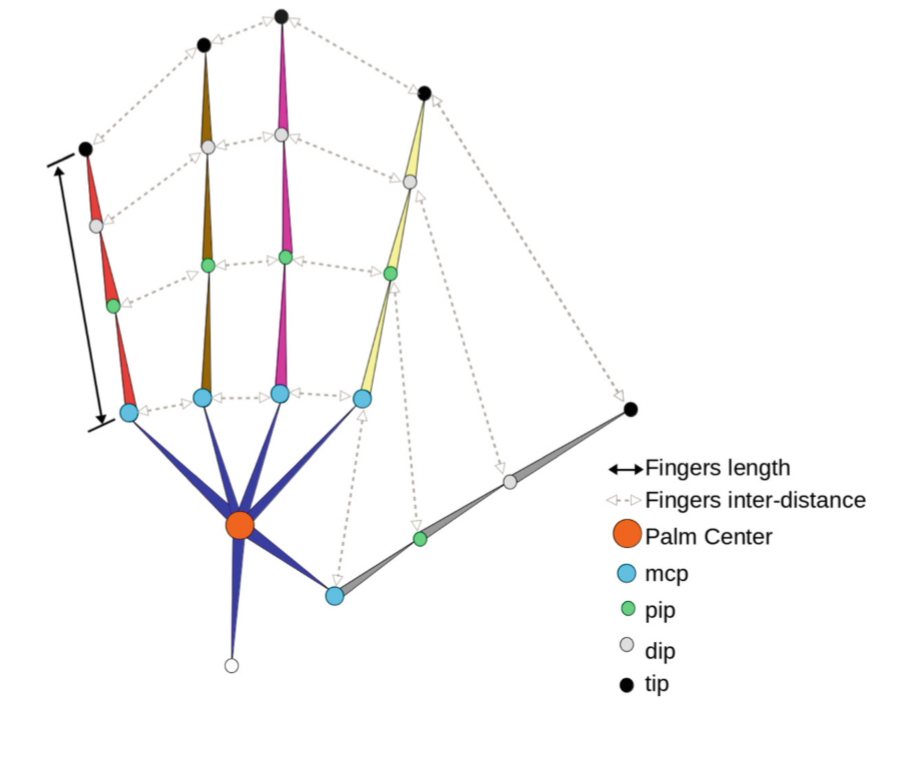
\includegraphics[width=0.7\linewidth]{Ressourcen/malik2018_hand_model}
		\caption[Handmodell nach \cite{Malik2018b}]{In \cite{Malik2018b} wird ein Modell ähnlich dem oben stehenden (Quelle: \cite{Malik2018b}) genutzt, in dem die vollständige Handpose durch 21, bzw. 22 (Gelenk-) Koordinaten bestimmt ist.}
		\label{fig:malik2018handmodel}
	\end{figure}
	
	
	\subsection{title}
	
	
\section{Kameraparameter}
\subsection{Intrinsische Parameter}
Die intrinsischen Paramter einer Kamera sind definiert durch die Brennweite $f$, das Format des Bildsensors und 
\subsection{Extrinsische Parameter}
	